%Copyright 2019 Christopher M. Jermaine (cmj4@rice.edu) and Risa B. Myers (rbm2@rice.edu)
%
%Licensed under the Apache License, Version 2.0 (the "License");
%you may not use this file except in compliance with the License.
%You may obtain a copy of the License at
%
%    https://www.apache.org/licenses/LICENSE-2.0
%
%Unless required by applicable law or agreed to in writing, software
%distributed under the License is distributed on an "AS IS" BASIS,
%WITHOUT WARRANTIES OR CONDITIONS OF ANY KIND, either express or implied.
%See the License for the specific language governing permissions and
%limitations under the License.
%===============================================================
\documentclass[aspectratio=169]{beamer}
\mode<presentation> 
{
\usetheme[noshadow, minimal,numbers,riceb,nonav]{Rice}
\usefonttheme[onlymath]{serif}
\setbeamercovered{transparent}
}
\useinnertheme{rectangles}

\usepackage[english]{babel}

\usepackage{mathptmx}
\usepackage{helvet}
\usepackage{courier}
\usepackage[T1]{fontenc}
\usepackage{trajan}
\usepackage{ textcomp }
\usepackage{listings}

\newenvironment{noindentitemize}
{ \begin{itemize}
 \setlength{\itemsep}{1.5ex}
  \setlength{\parsep}{0pt}   
  \setlength{\parskip}{0pt}
 \addtolength{\leftskip}{-2em}
 }
{ \end{itemize} }

\newenvironment{noindentitemize2}
{ \begin{itemize}
  \setlength{\itemsep}{0ex}
  \setlength{\parskip}{0pt}
  \setlength{\parsep}{0pt}   
  \addtolength{\leftskip}{-2em}  }
{ \end{itemize} }



\lstnewenvironment{SQL}
  {\lstset{
        aboveskip=5pt,
        belowskip=5pt,
        escapechar=!,
        mathescape=true,
        upquote=true,
        language=SQL,
        basicstyle=\linespread{0.94}\ttfamily\footnotesize,
        morekeywords={PRINT, CURSOR, OPEN, FETCH, CLOSE, DECLARE, BEGIN, END, PROCEDURE, FOR, EACH, WITH, PARTITION, 	TEST, WHETHER, PROBABILITY, OUT,LOOP,IF,CONTINUE, HANDLER,CALL, FUNCTION, RETURNS, LANGUAGE,BODY,RETURN, REPLACE,plpgsql,
        RAISE, NOTICE,
        REPLACE, ROW, BEFORE, EXIT, TEXT, REFCURSOR, QUOTE_LITERAL, DELIMITER,CONCAT,FOUND,LEAVE },
        deletekeywords={VALUE, PRIOR},
        showstringspaces=true}
        \vspace{0pt}%
        \noindent\minipage{0.65\textwidth}}
  {\endminipage\vspace{0pt}}
  
  
\lstnewenvironment{SQLtiny}
  {\lstset{
        aboveskip=5pt,
        belowskip=5pt,
        escapechar=!,
        mathescape=true,
        upquote=true,
        language=SQL,
        basicstyle=\linespread{0.94}\ttfamily\tiny,
        morekeywords={PRINT, CURSOR, OPEN, FETCH, CLOSE, DECLARE, BEGIN, END, PROCEDURE, FOR, EACH, WITH, PARTITION, 	TEST, WHETHER, PROBABILITY, OUT,LOOP,IF,CONTINUE, HANDLER,CALL, FUNCTION, RETURNS, LANGUAGE,BODY,RETURN, REPLACE,plpgsql,
        RAISE, NOTICE,
        REPLACE, ROW, BEFORE, EXIT, TEXT, REFCURSOR, QUOTE_LITERAL, DELIMITER,CONCAT,FOUND,LEAVE },
       deletekeywords={VALUE, PRIOR},
        showstringspaces=true}
        \vspace{0pt}%
        \noindent\minipage{0.47\textwidth}}
  {\endminipage\vspace{0pt}}

%===============================================================%

\title[]
{Tools \& Models for Data Science}

\subtitle{Optimization--Newton's Method}

\author[]{Chris Jermaine \& Risa Myers}
\institute
{
  Rice University 
}

\date[]{}

\subject{Beamer}


\begin{document}

\begin{frame}
 \titlepage
\end{frame}

%***********************************************************
\begin{frame}{Gradient Descent}

\begin{enumerate}
\item Goal: Find the parameter values for a model that best fit our data
\item Find the best direction to go in
\item Take a [sized] step in that best direction
\item Repeat until convergence
\end{enumerate}
\end{frame}
%***********************************************************
\begin{frame}{Alternatives to Gradient Descent}

\begin{itemize}
        \item Gradient descent is great
        \begin{itemize}
                \item Easy to use
		\item Widely applicable
		\item But convergence can be slow
        \end{itemize}
	\item Can we do better?  Sure!
\end{itemize}
\end{frame}
%***********************************************************
\begin{frame}{Second-Order Methods}

\begin{itemize}
\item Class of iterative optimization methods
	\begin{itemize}
	\item Use not only first partial derivatives
	\item But second as well
	\item Speeds convergence
	\item Cost: more complexity
	\item Cost: quadratic in number of variables 
	\end{itemize}
\end{itemize}
\end{frame}
%***********************************************************
\begin{frame}{Newton's Method}

\begin{itemize}
\item Classic second order method for optimization\footnote {second order method means it uses the second derivative} 
\item Comes from Newton's method for finding zero of a function $F()$ 
\item Recall that the ``zeroes'' of a function are the roots / solutions
\item Use this approach to keep finding better approximations to the zeros of a function
\end{itemize}
\end{frame}
%***********************************************************
\begin{frame}{Roadmap}

\begin{enumerate}
	\item Review of Newton's method for finding the root of a \textbf{1 variable function}
	\item Introduce method for finding the root of a \textbf{1 variable gradient of a Loss function}
	\item Review of Newton's method for finding the root of a \textbf{multi-variable function}
	\item Introduce method for finding the root of a \textbf{multi-variable gradient of a Loss function}
\end{enumerate}
\end{frame}
%***********************************************************
\begin{frame}[fragile]{Newton's Method - Refresher}

\begin{columns}[T]
\begin{column}{0.5\textwidth}
\begin{SQL}
$\theta \leftarrow$ intial guess;
while $\theta$ keeps changing, do:
  $\theta \leftarrow \theta - F'(\theta)^{-1}F(\theta)$; 
\end{SQL}
\end{column}
\begin{column}{0.5\textwidth}
\begin{itemize}
\item Make an initial guess
\item Approximate $F(\theta)$ with a  line (tangent to $F()$ at that guess) %Solve for the zero of the linear approximation to estimate the root, $\theta$
\item Update $\theta$
\end{itemize}
\end{column}
\end{columns}
\begin{noindentitemize}
\item $\theta$ is the value of the model parameter
%\item 
\end{noindentitemize}
\end{frame}

%***********************************************************
\begin{frame}{Newton's Method Intuition}

\begin{columns}[T]
\begin{column}{0.65\textwidth}
\begin{enumerate}
\item Pick a value for $\theta$
\item Evaluate $F(\theta)$
\item Evaluate the derivative of the function at $\theta$, $F'(\theta)$
\item Revise $\theta$ based on these values
\item Repeat until convergence of $\theta$
\end{enumerate}
\end{column}
\begin{column}{0.35\textwidth}
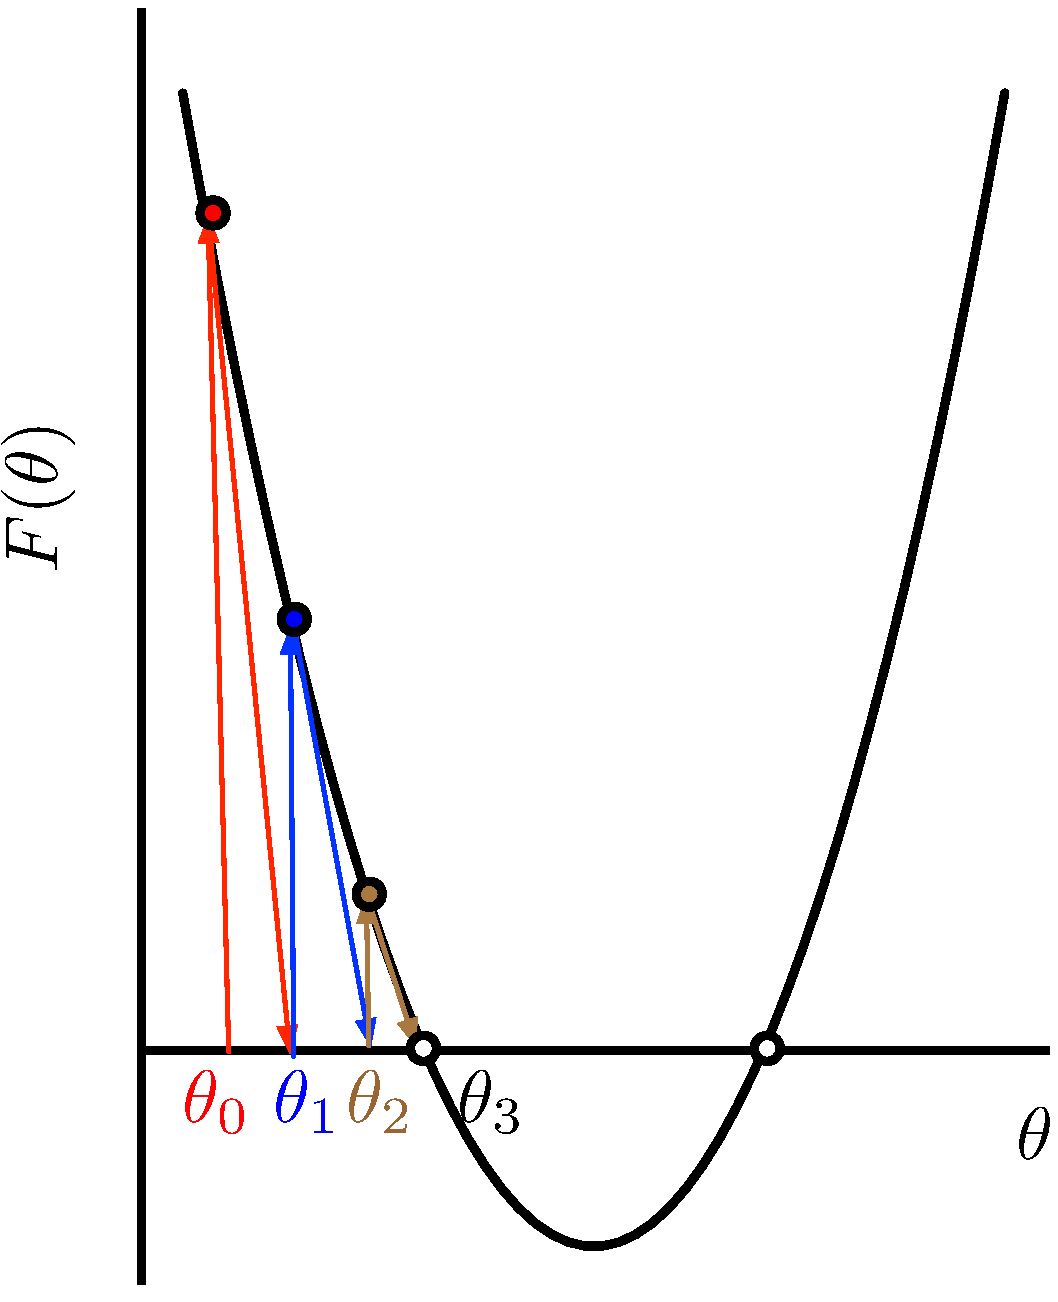
\includegraphics[width=1\textwidth]{lectNM/newtonV3.pdf}
\end{column}
\end{columns}
\end{frame}

%***********************************************************
\begin{frame}{Isn't that what we did in Gradient Descent?}

\begin{columns}[T]
\begin{column}{0.65\textwidth}
Key difference:
\begin{itemize}
\item Root finding, not minimum finding
\item Want the zero of the \textbf{function}
\item Not the zero of the \textbf{derivative}
\end{itemize}
\end{column}
\begin{column}{0.35\textwidth}
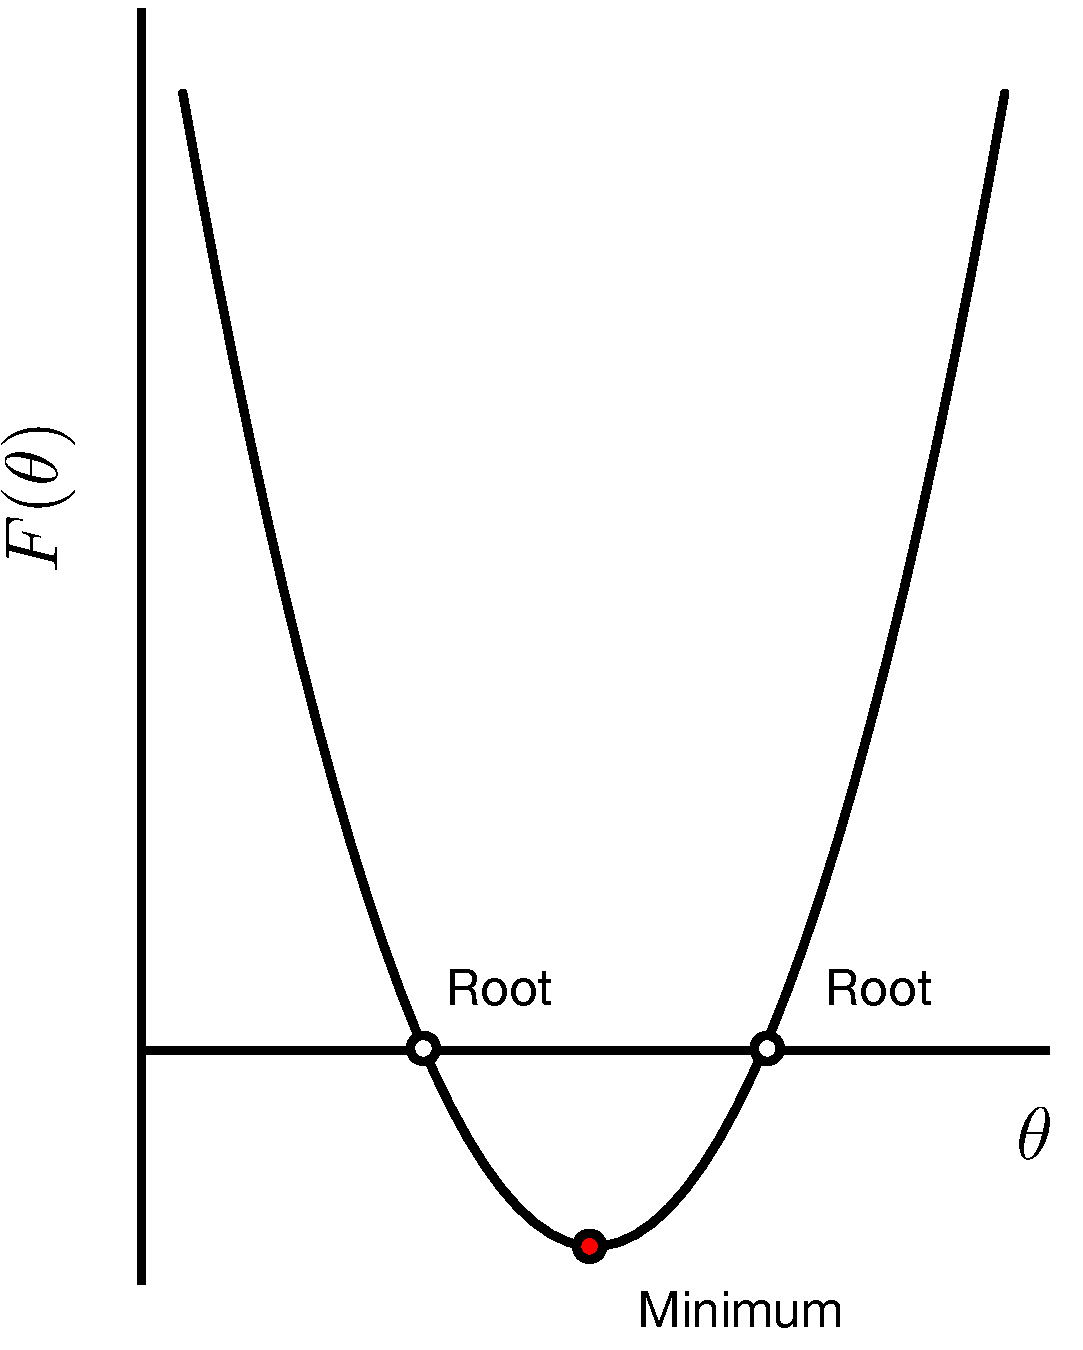
\includegraphics[width=1\textwidth]{lectNM/rootVsMin.pdf}
\end{column}
\end{columns}
\end{frame}
%***********************************************************
\begin{frame}[fragile]{Netwon's Method for Optimization}

\begin{itemize}
\item In data science, don't want a zero
	\begin{itemize}
	\item We want a max/min of loss function $L()$
	\item So, just find the root (zero) of the derivative $L'()$
	\item So, $F(\theta) \rightarrow L'(\theta)$
	\end{itemize}
\item Algorithm becomes:
\end{itemize}
\begin{SQL}
$\theta \leftarrow$ intial guess;
while $\theta$ keeps changing, do:
  $\theta \leftarrow \theta - \frac{L'(\theta)}{L''(\theta)}$;
\end{SQL}
\end{frame}
%***********************************************************
\begin{frame}{Multi-Variate Newton's Method}

\begin{itemize}
\item Say we have a multi-variate function $F: \mathbb{R}^d \rightarrow \mathbb{R}^d$, where $d$ is the number of dimensions
\begin{itemize}
	\item The $i$th output of $F$ is given by the function $F_i$
	\item So $F(\Theta) = \langle F_1(\Theta), F_2(\Theta), ..., F_d(\Theta)\rangle$ % \Theta is a vector
\end{itemize}
\item We want to find a zero of $F$; that is, find $\Theta = \langle \theta_1, \theta_2, ..., \theta_d \rangle$ such that:
\begin{align}
F_1 &(\theta_1, \theta_2, ..., \theta_d) = 0 \nonumber \\
F_2 &(\theta_1, \theta_2, ..., \theta_d) = 0 \nonumber \\
&... \nonumber \\
F_d &(\theta_1, \theta_2, ..., \theta_d) = 0 \nonumber
\end{align}
\item How to do this?
\end{itemize}
\end{frame}
%***********************************************************
\begin{frame}{Multi-Variate Newton's Method}

\begin{itemize}
\item Turns out it's not so difficult...
	\begin{itemize}
	\item Won't do the derivation (relies on multi-variate Taylor expansion)
	\item From Linear Algebra: a Jacobian Matrix contains all the partial first derivatives of a function
	\item Here, $F_i$ is the function that governs the $i$th dimension
	\item Define the ``Jacobian'' of $F$ to be:
	$$ J_F = \left( \begin{array}{cccc}
	\frac{\partial F_1}{\partial \theta_1} & \frac{\partial F_1}{\partial \theta_2} & \frac{\partial F_1}{\partial \theta_3} & ... \\
	\frac{\partial F_2}{\partial \theta_1} & \frac{\partial F_2}{\partial \theta_2} & \frac{\partial F_2}{\partial \theta_3} & ... \\
	\frac{\partial F_3}{\partial \theta_1} & \frac{\partial F_3}{\partial \theta_2} & \frac{\partial F_3}{\partial \theta_3} & ... \\
	... & ... & ... & ... 
	 \end{array} \right)$$
	\item Note: this is a $d \times d$ matrix of functions!
	\item Rows cover the different parameters for a single dimension
	\item Columns cover the value of $F$ for each dimension for a single parameter
	\item We can evaluate it at any set of parameter values
	\item So $J_F(\Theta)$ is a matrix of scalars
	\end{itemize}
\end{itemize}

\end{frame}
%***********************************************************
\begin{frame}[fragile]{Multi-Variate Newton's Method}

\begin{noindentitemize}
\item Multi-Variate Newton's is simply:
\end{noindentitemize}
\begin{SQL}
$\Theta \leftarrow$ intial guess;
while $\Theta$ keeps changing, do:
  $\Theta \leftarrow \Theta - J_F^{-1}(\Theta)F(\Theta)$;
\end{SQL}
\begin{noindentitemize}
\item Update each model parameter using the inverse of the Jacobian evaluated at the current values of the model parameters, $\Theta$, and the value of the function using the same parameters
%\item Computable using numpy, once you have the partial derivatives
\end{noindentitemize}
\end{frame}
%***********************************************************
\begin{frame}{What About Multi-Variate Optimization?}

\begin{itemize}
\item Again, we want to solve an optimization problem, not find function roots
\item Difference: we don't have a system of equations to solve
\item In multidimensional space, this is equivalent to standing at the top of a mountain or bottom of a valley
	\begin{itemize}
	\item Just have a loss function $L()$, which we want to minimize (or maximize)
	\item Min/max is at $\Theta$ such that:
	\begin{align}
	\frac{\partial L}{\partial \theta_1}(\Theta) &= 0 \nonumber \\
	\frac{\partial L}{\partial \theta_2}(\Theta) &= 0 \nonumber \\
         &... \nonumber \\
	\frac{\partial L}{\partial \theta_d}(\Theta) &= 0 \nonumber 
	\end{align}
	\item That is, we want $\Theta$ such that $\nabla L(\Theta) = \langle 0, 0, ..., 0 \rangle$
	\item Can then use exactly the same algorithm as before [MV Newton's Method] to find root of $\nabla L(\Theta)$ %next slide
	\end{itemize}
\end{itemize}
\end{frame}
%***********************************************************
\begin{frame}[fragile]{Multi-Variate Optimization}

To find max/min, then this:

\begin{SQL}
$\Theta \leftarrow$ intial guess;
while $\Theta$ keeps changing, do:
  $\Theta \leftarrow \Theta - J_F^{-1}(\Theta)F(\Theta)$;
\end{SQL}

Becomes this:

\begin{SQL}
$\Theta \leftarrow$ intial guess;
while $\Theta$ keeps changing, do:
  $\Theta \leftarrow \Theta - J_{\nabla L}^{-1}(\Theta)\nabla L(\Theta)$;
\end{SQL}


\begin{itemize}
\item We are taking the Jacobian over the gradient instead of over a system of equations, $F_i$
\end{itemize}

\end{frame}
%***********************************************************
\begin{frame}[fragile]{One Last Thing}

We have:

\begin{SQL}
$\Theta \leftarrow$ intial guess;
while $\Theta$ keeps changing, do:
  $\Theta \leftarrow \Theta - J_{\nabla L}^{-1}(\Theta)\nabla L(\Theta)$;
\end{SQL}

\begin{itemize}
\item The matrix of functions $J_{\nabla L}$ is typically called the ``Hessian'' of $L$
\item Entries are:
	$$ H_L = \left( \begin{array}{cccc}
	\frac{\partial L}{\partial \theta_1^2} & \frac{\partial L}{\partial \theta_1 \partial \theta_2} & \frac{\partial L}{\partial \theta_1 \partial \theta_3} & ... \\
	\frac{\partial L}{\partial \theta_1 \partial \theta_2} & \frac{\partial L}{\partial \theta_2^2} & \frac{\partial L}{\partial \theta_2 \partial \theta_3} & ... \\
	\frac{\partial L}{\partial \theta_1 \partial \theta_3} & \frac{\partial L}{\partial \theta_2 \partial \theta_3} & \frac{\partial L}{\partial \theta_3^2} & ... \\
	... & ... & ... & ... 
	 \end{array} \right)$$
\item Each entry is the 2nd derivative of the loss function with respect to each parameter
\item Each row is the Jacobian given a set of model parameters, $\Theta$
\end{itemize}
\end{frame}
%***********************************************************
\begin{frame}{Pros and Cons of Newton's}

\begin{itemize}
\item Pro: Convergence is quadratic; that is, error decreases quadratically
\item Pro: Hundreds/thousands of iterations (gradient descent) becomes tens
\item Pro: No learning rate to set
\item Pro: Doesn't require $F(\Theta)$ to be convex
\item[]
\item Con: More complicated than gradient descent!
%\item Con: Solution can depend on starting guess - TRUE for all of these class of methods
\item Con: quadratic cost each iteration (linear gradient descent)
\item[] The Hessian is quadratic in the number of variables
\item Actually, the cost is worse than quadratic, since the matrix has to be inverted 
\item Con: The second derivative has to exist
\end{itemize}
\end{frame}
%***********************************************************
\begin{frame}{In Practice}

\begin{itemize}
\item Not used much in practice since in high dimensions, $d \times d$ is too big
\item Usable for < 100K parameters, really hard at 1M
\item Quasi-Newton methods are used instead
\item Typically use just a portion or estimation of the Hessian matrix
\item E.g. Limited-memory BFGS
\end{itemize}
\end{frame}
%***********************************************************
\begin{frame}{Questions?}
\begin{itemize}
	\item[?] What do we know now that we didn't know before?
	\vspace{2em}
	\item[?] How can we use what we learned today?
\end{itemize}
\end{frame}

%***********************************************************
\begin{frame}{Questions?}
\begin{itemize}
	\item What do we know now that we didn't know before?
	\begin{itemize}
	\item We have another numerical method to find the parameters of a loss function
	\item We understand how we can handle multi-dimensional data
	\end{itemize}

	\item How can we use what we learned today?
	\begin{itemize}
	\item We can  find the model parameters using a different approach
	\end{itemize}
\end{itemize}
\end{frame}


\end{document}
